%!TEX root = ../prueba.tex
En este capítulo se describe la arquitectura utilizada para la construcción y operación del sistema. Se hará uso de diagramas y algunas referencias bibliográficas para permitir el entendimiento adecuado de algunos conceptos formales.

\section{Arquitectura Física}

En esta sección se realizar la especificación técnica y física de la arquitectura sobre la cual la aplicación y el sistema funcionaran desde su puesta en producción. Dicha especificación se realiza utilizando como base la figura \ref{fig:arqFisica}.

\begin{figure}[hbtp!]
	\begin{center}
		\fbox{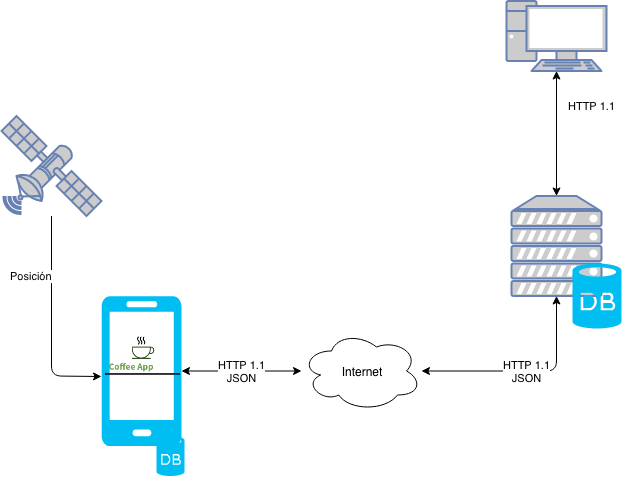
\includegraphics[width=.5\textwidth]{img/arqFisica}}
		\caption{Arquitectura Física del Sistema}
		\label{fig:arqFisica}
	\end{center}
\end{figure}

\subsection{Arquitectura Base}
El sistema está pensado para trabajar bajo un esquema centralizado tomando como base la arquitectura \textbf{Cliente-Servidor}. Esta arquitectura nos sirve como punto de partida debido a dos principales razones:
	\begin{itemize}
		\item Es requerido un punto centralizado(servidor) donde se almacene la mayor cantidad de información y que sea un punto de acceso para varios dispositivos.
		\item Es requerido hacer la implementación de dos diferentes clientes desde los cuales se tendrá acceso al servidor y por consiguiente a la información. El primer cliente consta de una aplicación móvil para dispositivos con sistema operativo Android, el segundo cliente consta de una aplicación web basada en \textit{Servlets} y \textit{JSP's}. 
	\end{itemize}

Se optó también por utilizar como base la arquitectura \textbf{Cliente - Servidor} ya que nos permite el uso del protocolo \textit{HTTP 1.1} para crear varios canales de comunicación entre los distintos clientes que accederán al sistema. El protocolo \textit{HTTP} nos define que para que exista comunicación entre el Cliente y el Servidor se debe hacer uso de dos mecanismos: una \textit{Petición} y una \textit{Respuesta}. A grandes rasgos, la petición está formada entre otras cosas por cabeceras, métodos y parámetros los cuales son enviados desde el cliente a través de la red hasta llegar al servidor el cual debe validar que la \textit{URL} desde la cual se hace la petición es válida. Posteriormente el servidor procesa la petición y en caso de existir el recurso y el método contenido en la petición le devolverá al cliente una respuesta con la información solicitada utilizando el formato indicado en el \textit{MIME/TYPE} de la respuesta.\\

Los actores que podrán acceder al sistema mediante la aplicación web son:
	\begin{itemize}
		\item El \getElementById[Stakeholder]{Jefe} dado que es el encargado de registrar, editar o eliminar la información de las cafeterías de las que es dueño así como sus respectivos locales y productos que se podrán encontrar en todos los locales de su franquicia.
		\item El \getElementById[Stakeholder]{Agente} dado que es el encargado de habilitar el acceso a las personas que tienen una cuenta bloqueada al sistema.
		\item El \getElementById[Stakeholder]{ResponsableDeLocal} dado que es el encargado de registrar la información de los productos que se ofertan en un local.
	\end{itemize}

Los actores que tendrán acceso a la aplicación móvil son:
	\begin{itemize}
		\item El \getElementById[Stakeholder]{Cliente} dado que desde su dispositivo únicamente podrá consultar información de las cafeterias, locales y productos publicados para realizar pedidos que serán atendidos por el personas de los locales, la aplicación móvil hará uso de dos mecanismos relevantes:
		\begin{itemize}
			\item El módulo GPS ya que cuando el cliente acceda a la aplicación se determinará su posición y con esto la ubicación de los locales más cercanos en un radio de 2 kilómetros.
			\item Una base de datos local que almacenará los pedidos que no han sido confirmados para que el cocinero de un local inicie su preparación.
		\end{itemize}
		\item El \getElementById[Stakeholder]{Cocinero} dado que a su tableta o a la tableta proporcionada por la cafetería, atenderá los pedidos e indicará la conclusión de su preparación para que se le entrege al cliente.
\end{itemize}

\subsection{Especificaciones Técnicas}
A continuación se especifican los detalles técnicos del sistema, es decir, el Hardware y Software requerido para que el sistema opere de forma estable.

\subsubsection{Servidor}
El servidor tiene las siguientes especificaciones:
	\begin{description}
		\item[Marca:]Servidor Dell PowerEdge T30.
		\item[Procesador:]Intel Xeon E3-1225V5 3.30GHz.
		\item[Memoria RAM:]8GB DDR4.
		\item[Disco Duro:]1TB.
		\item[Sistema Operativo:] CentOS 7.4-1708.
	\end{description}

\subsection{Base de Datos}
	\begin{description}
		\item[SGBD:] Postgresql 9.4
	\end{description}

\subsubsection{Cliente Web}
La aplicación web puede ser utilizada bajo las siguientes especificaciones:
	\begin{description}
		\item[Navegadores Compatibles:]\hspace{0.5pt}
			\begin{itemize}
				\item Google Chrome Versión $\geq$ 70.0.3538.
				\item Mozilla Firefox $\geq$ 63.0.
				\item Safari $\geq$ 12.0.
			\end{itemize}
		\item[Resolución:]\hspace{0.5pt}
			\begin{itemize}
				\item Mínima:1027x768
				\item Máxima:1920x1080
			\end{itemize}
	\end{description}

\subsubsection{Cliente Móvil}
La aplicación móvil puede ser utilizada bajo las siguientes especificaciones:
	\begin{description}
		\item[Sistema Operativo:] Android >= 5.0 Lollipop.
		\item[Memoria RAM:] 2GB.
		\item[Almacenamiento:] 16 GB.
	\end{description}


\subsection{Arquitectura Lógica}
Una vez descrita la arquitectura física del sistema, es requerido indicar y especificar cómo será construido. En general las aplicaciones que se van a desarrollar utilizarán una arquitectura a capas. En la figura \ref{fig:arqLogica} se pueden observar las capas del sistema en los diferentes clientes(o aplicaciones) y posteriormente se hará una descripción de la función de cada capa.\\

\begin{figure}[hbtp!]
	\begin{center}
		\fbox{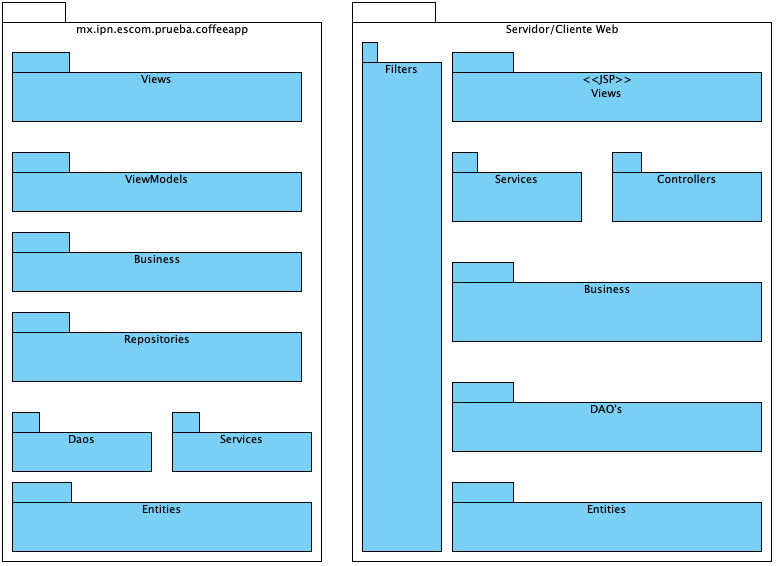
\includegraphics[width=0.8\textwidth]{img/arqLogicaP}}
		\caption{Arquitectura Lógica del Sistema}
		\label{fig:arqLogica}
	\end{center}
\end{figure}

\subsubsection{Arquitectura Lógica del Servidor/Aplicación Web}
Como se mencionó al iniciar esta sección, las aplicaciones están construidas a partir de una arquitectura multi capa.El servidor(paquete del lado derecho en la figura \ref{fig:arqLogica}) está dividido en las siguientes capas:
	\begin{description}
		\item[Entities:] En esta capa se definen las clases que se utilizarán para la manipulación de las estructuras de datos de la base de datos.
		\item[DAO's:] En esta capa se definen las clases que sirven de interacción entre la capa de \textit{business} y la capa de \textit{entities} para la recolección de datos utilizando el patrón de diseño DAO.
		\item[Business:] En esta capa se definen las clases que sirven para la abstracción de las reglas de negocio así como de las operaciones y funciones disponibles en el sistema.
		\item[Services:] En esta capa se definen las clases que corresponden al servicio RESTful que será consumido por la aplicación móvil.
		\item[Controllers:] Está capa tiene el propósito establecido para la capa de \textit{Controlador} en el patrón de diseño \textit{MVC} en donde se va a administrar el flujo de datos que hay entre la capa \textit{views} y la capa \textit{business}.
		\item[Views:] Está capa contiene los archivos JPA's que presentan las interfaces de usuario para la aplicación web.
	\end{description}
	
Como observación general, en el paquete de \textit{Business} se creará una clase que lleva por nombre \textit{GenericBs} el cual se compone de otra clase en el paquete \textit{DAO's} que lleva por nombre \textit{GenericDao}, esta última clase implementa los métodos genéricos para actualizar, guardar o encontrar una entidad en la base de datos, por esta razón todas las clases que se encuentren en un paquete con terminación \textit{bs} heredan de la clase \textit{GenericBs}.\\
	
En la figura \ref{fig:maqservarq} se presenta un diagrama de clases que tiene como principal propósito mostrar las clases y paquetes que se implementarán para el módulo de autenticación y usuarios.

\begin{figure}[hbtp!]
	\begin{center}
		\fbox{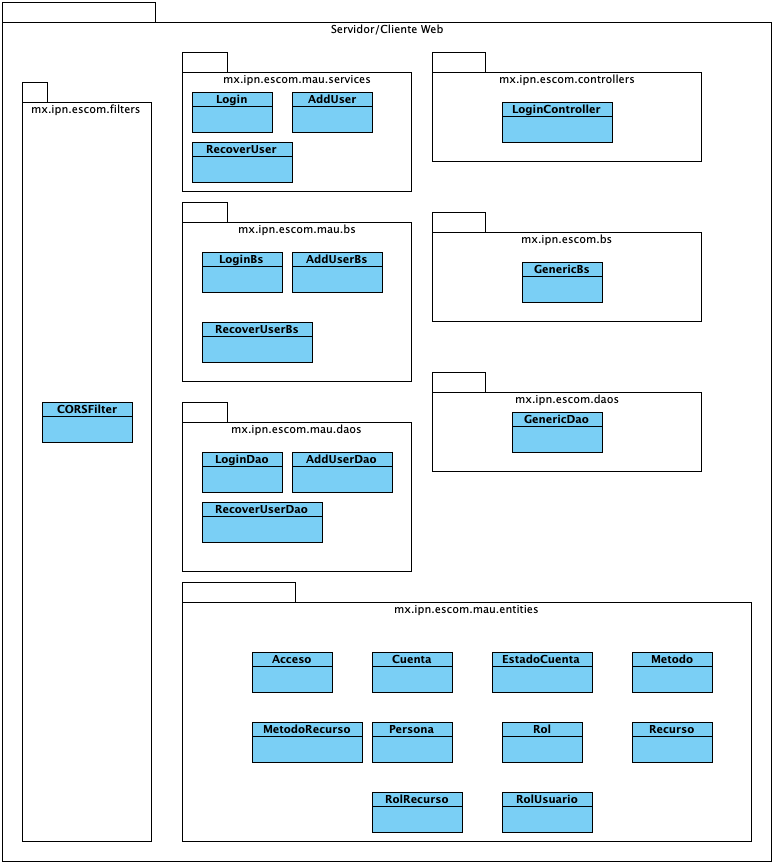
\includegraphics[width=0.8\textwidth]{img/MAU_SERV_ARQ}}
		\caption{Arquitectura Lógica en el Servidor del Módulo de Autenticación y Usuarios.}
		\label{fig:maqservarq}
	\end{center}
\end{figure}

	
\subsubsection{Arquitectura Lógica de la Aplicación Móvil}
La aplicación móvil se va a construir con base en el patrón arquitectónico \textit{MVC}, agregando una capa la cual tiene como principal propósito administrar las peticiones que se van a mandar al servidor y proveer de datos a la capa de \textit{Models}. Estas capas se pueden observar en la figura \ref{fig:arqLogica} del lado izquierdo en el paquete de Cliente Móvil. Así mismo dado que la aplicación móvil es nativa del sistema operativo Android, se hará uso de algunos patrones de diseño establecidos por \textit{Google} para el comportamiento de algunos componentes como lo es el patrón \textit{Adapter} para el componente \textit{Recycler View}. A continuación se hace la descripción de las capas del patrón MVVM:
	\begin{description}
		\item[Views:] En este paquete se encuentran aquellas clases que construyen las interfaces de usuario y se actualizan con respecto a los eventos o cambios de datos de la capa \textit{ViewModel}.
		\item[ViewModels:] En este paquete se encuentran las clases que identifican un cambio en el modelo y actualizan la interfaz.
		\item[Business:] En este paquete se encuentran las clases que abstraen e implementan algunas de las reglas de negocio que intervienen directamente con el éxito o fracaso de una operación en el sistema.
		\item[Repositories:] En este paquete se encuentran las clases que permiten la conexión a la base de datos local o realizar la conexión con el servicio web para la búsqueda e inserción de datos.
		\item[Daos:] En este paquete se encuentran las clases que, de acuerdo con el patrón de diseño \textit{DAO}, permite el acceso a los datos almacenados en el dispositivo de forma local.
		\item[Services:] En este paquete se encuentran las clases que permiten la conexión al servidor para la recolección e inserción de datos en el sistema.
		\item[Entities:] En este paquete se encuentran las clases que abstraen las entidades de negocio que se muestran al cliente o se insertan en el sistema.
	\end{description}


\begin{figure}[hbtp!]
	\begin{center}
		\fbox{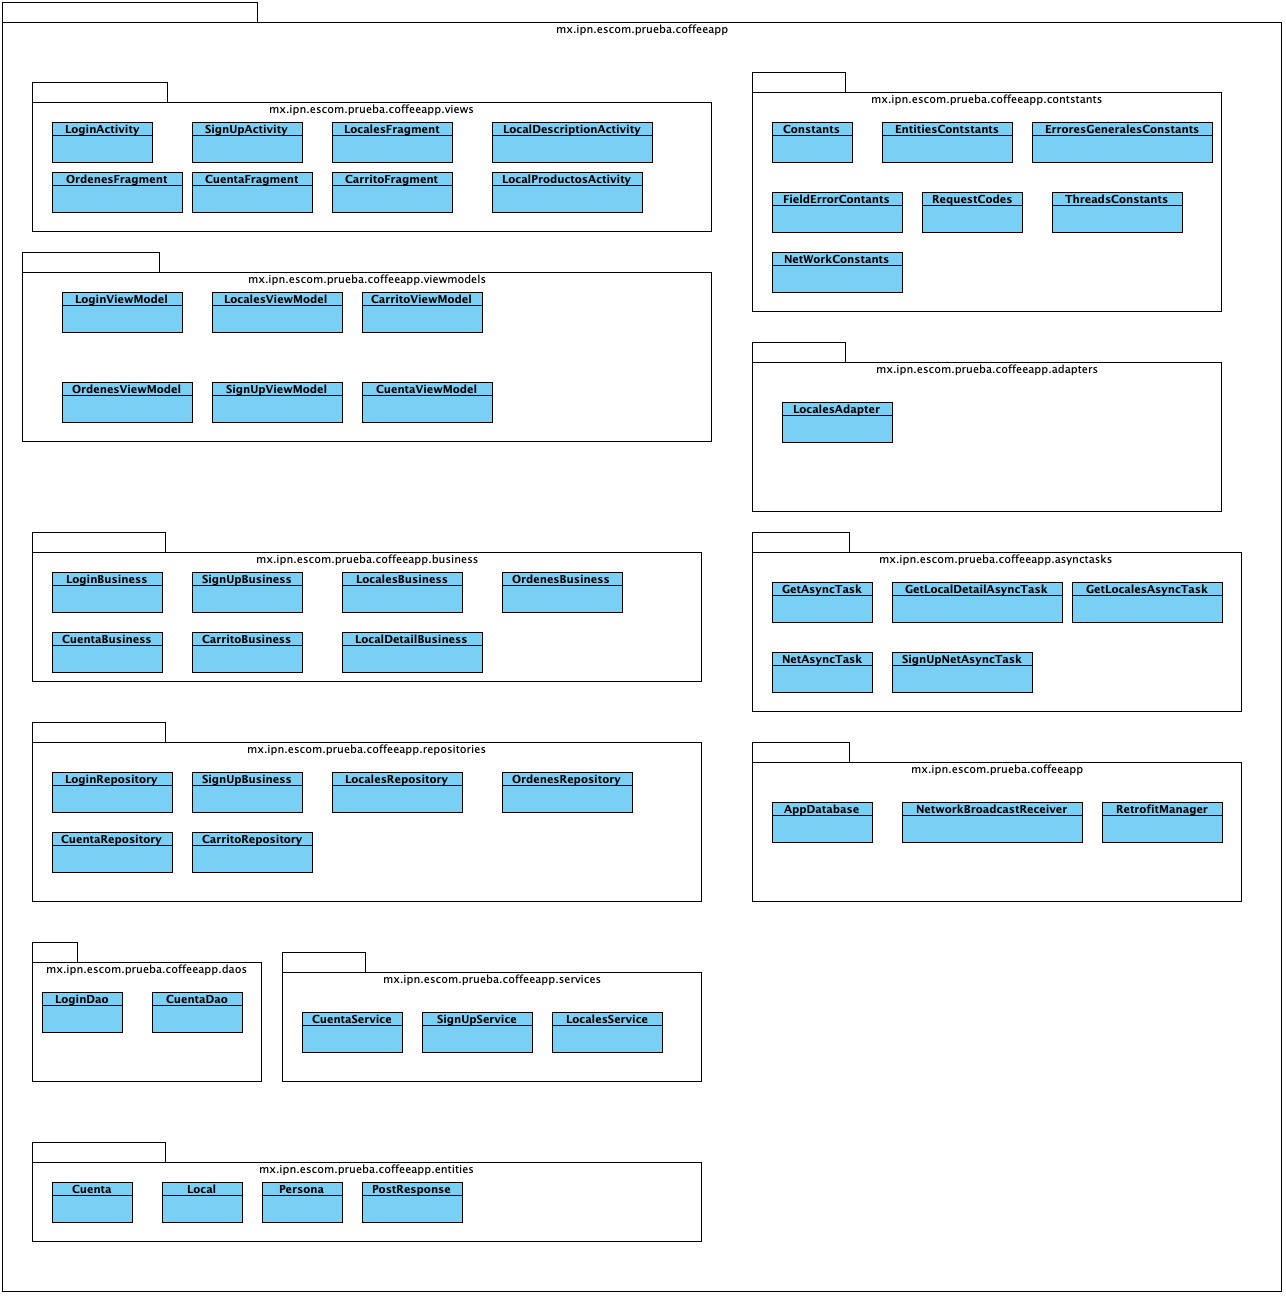
\includegraphics[width=\textwidth]{img/APP_ARQ}}
		\caption{Arquitectura Lógica de la Aplicación Móvil}
		\label{fig:arqLogApp}
	\end{center}
\end{figure}


